\documentclass[10pt,a4paper]{article}
\usepackage[textwidth=18cm,textheight=25cm]{geometry}
\usepackage[pdftex]{graphicx}
\usepackage{multirow}
% cv-custom.tex
%
% Custom macro commands and packages
% for formatting a Curriculum Vitae.
%
% Author: Matthew Earnshaw <matt@earnshaw.org.uk>
% Inspired by http://www.cv-templates.info/2009/03/professional-cv-latex/

\pagestyle{empty}

% Packages
\usepackage[usenames,dvipsnames]{color} % For custom colours
\usepackage{titlesec} % For custom section headings
\usepackage{mdwlist} % For compact lists
\usepackage[pdftex]{hyperref}
\usepackage{marvosym} % For icons

% Hyperlink colour and style
\definecolor{linkcolour}{rgb}{0,0.2,0.6}
\hypersetup{colorlinks,breaklinks, urlcolor=linkcolour, linkcolor=linkcolour}

% Custom colour
\definecolor{lgray}{gray}{0.4}

% Custom list bullet
\renewcommand{\labelitemi}{$\succ$}

% Header commands
\newcommand{\name}[1]{\LARGE\textbf{#1}}
\newcommand{\address}[1]{\color{lgray}{#1}}
\newcommand{\tel}[1]{\Large\Telefon~\small{#1}}
\newcommand{\email}[1]{\Large\Letter~\href{mailto:#1}{\small{#1}}}
\newcommand{\web}[2]{\Large\Mundus~\href{#1}{\small{#2}}}
	
% Section headings
\titleformat{\section}{\large\scshape\raggedright}{}{0em}{}[\titlerule]
\titlespacing{\section}{0pt}{0.6cm}{5pt}
% Note: Create an environment for sections ?

% Full width tables
\newenvironment{ftabular}[1]
{\begin{tabular*}{0.95\textwidth}{@{\extracolsep{\fill}}#1}}
{\end{tabular*}}

\usepackage[utf8]{inputenc}

\begin{document}
\footnotesize
\fontfamily{ptm}

\section{\sc K{\footnotesize İŞ\footnotesize İSEL} B{\footnotesize İLG\footnotesize İLER}}

\begin{tabular}{ l l l }
\vspace{0.5 mm}\\
\multirow{8}{*}{\fbox{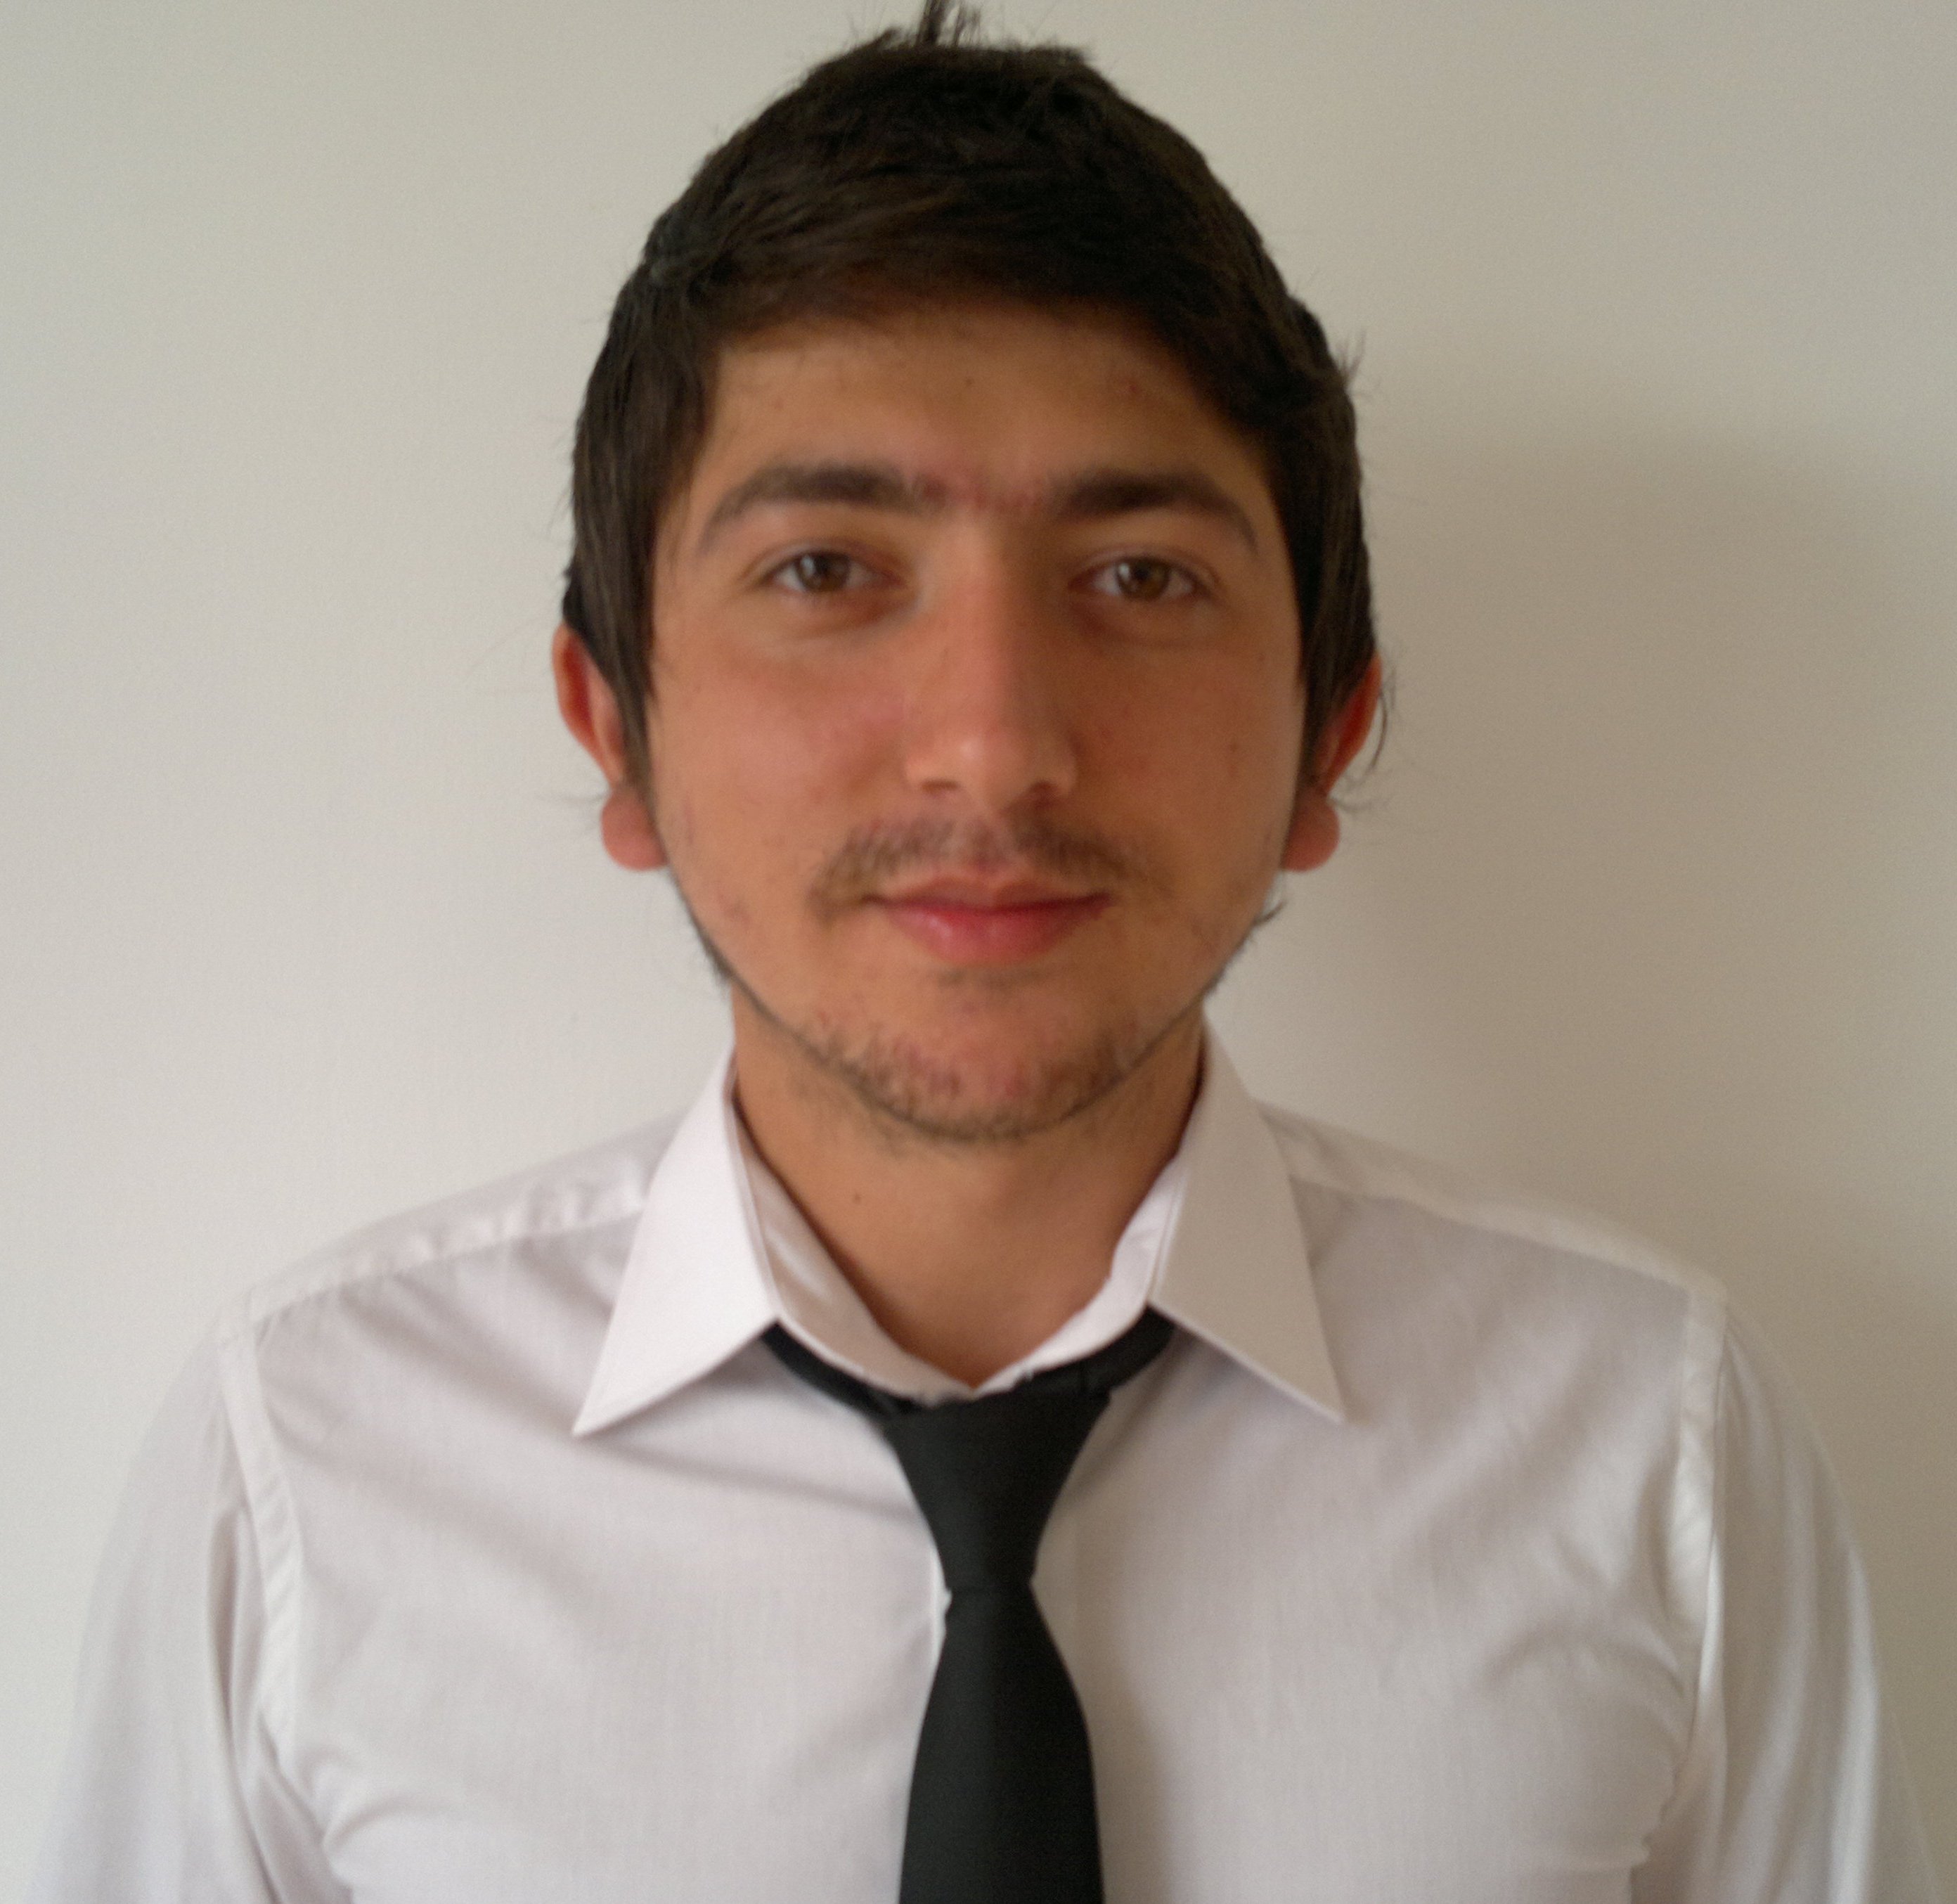
\includegraphics[height=25mm,width=25mm]{semih.jpg}}}
& {\Huge\name{Semih  Özköroğlu}}& Tarih: \small{08/11/2012}\\
\vspace{1 mm}\\
& \textbf{Adres :} \address{Güven mah. Taşlık sok. No:21 Daire:4 Güngören/İSTANBUL} & \web{http://sozkoroglu.me}{sozkoroglu.me}\\
& \textbf{Doğum Tarihi :} \address{18.11.1989} & \email{sem@bil.omu.edu.tr}\\
& \textbf{Medeni Hal :} \address{Bekar} & \tel{0506 3474727}\\
& \textbf{Askerlik Durumu  :} \address{Tecilli 01.08.2014} & \\
& \textbf{Engellilik Durumu :} \address{Hayır} & \\
\end{tabular}

\section{\sc E{\footnotesize Ğ\footnotesize İT\footnotesize İM} B{\footnotesize İLG\footnotesize İLER\footnotesize İ}}
\hspace*{1.6in}\begin{tabular}{lr}
\vspace{0.5 mm}\\
\textbf{Eğitim Seviyesi :} & Üniversite /\textbf{3.lük derecesi ile Mezun} \\
\vspace{0.5 mm}\\
\textbf{Üniversite :} & Samsun 19 Mayıs Üniversitesi \\
\textbf{Fakülte/Enstitü :} & Mühendislik Fakültesi \\
\textbf{Bölüm :} & Bilgisayar Mühendisliği \\
\textbf{Öğrenim Tipi / Dili :} & Türkçe / Örgün Öğretim\\
\textbf{Not Sist. / Mez. Derecesi :} & 100 / 77.31 \\
\textbf{Başlama / Mez. Tarihi :} & Eylül -2009 / Haziran -2012\\
\vspace{0.5 mm}\\
\textbf{Lise Türü / Bölüm :} & Düz Lise / Fen\\
\textbf{Öğrenim Tipi / Dili :} & Örgün Öğretim / Türkçe\\
\textbf{Lise Adı :} & izzet ünver\\
\textbf{Not Sist. / Mez. Derecesi :} & 100 / 83.50\\
\textbf{Başlama / Mez. Tarihi :} & Eylül - 2004 / Haziran-2007\\
\vspace{0.5 mm}\\
\end{tabular}

\underline{\textbf{Yabancı Diller}}
\vspace{0.5 mm}\\
\begin{itemize}
  \item{\textbf{Dil :} ingilizce}
  \begin{itemize}
    \item{\textbf{Genel :} orta}
    \item{\textbf{Okuma :} iyi}
    \item{\textbf{Yazma :} orta}
    \item{\textbf{Konuşma :} başlangıç}
  \end{itemize}
\end{itemize}

\section{\sc İ{\footnotesize Ş} D{\footnotesize ENEY\footnotesize İM\footnotesize İ}}
\begin{ftabular}{r|p{14cm}}
\textsc{Kasım – 2011} & \textbf{Omü mühendislik fakültesi - Samsun} \\
\vspace{0.5 mm}\\
 & \textbf{Sektör – Bölüm Pozisyon :} Bilgisayar / BT / Internet - Bakım Onarım - Yönetici Asistanı\\
 & \textbf{İşin Tanımı :} Wordpress tabanlı mühendislik fakültesi web servisinin bakımı, güncellenmesi, tasarımı gibi konularda çalışma yapmaktaydım\\
 & \textbf{Ayrılma Nedeni :} Okuldan mezun oldum\\

\multicolumn{2}{c}{ } \\ % Spacer 

\textsc{Ek{\footnotesize İ}m-2010 Haz{\footnotesize İ}ran-2011} & \textbf{Omü endüstri mühendisliği – Samsun} \\
\vspace{0.5 mm}\\
 & \textbf{Sektör – Bölüm Pozisyon :} Bilgisayar / BT / Internet - Bilgi Teknolojileri - Bilgisayar Mühendisi\\
 & \textbf{İşin Tanımı :} Endüstri mühendisliği bölümünde bilgisayar bakımı,ağ bağlantıları kontrolü , Web sitesi tasarımı\\

\multicolumn{2}{c}{ } \\ % Spacer 

\textsc{Kasım-2009 Haz{\footnotesize İ}ran-2010} & \textbf{Omü uzaktan eğitim merkezi - Samsun} \\
\vspace{0.5 mm}\\
 & \textbf{Sektör – Bölüm Pozisyon :} Eğitim - Bilgisayar Mühendisi\\
 & \textbf{İşin Tanımı :} Ebelik lisans tamamlama programında ebelere internet üzerinden ders verilmekte ,
Burada video işleme ve destek bölümünde yer aldım\\

\multicolumn{2}{c}{ } \\ % Spacer 

\textsc{Temmuz-2011} & \textbf{Dsmart - {\footnotesize İ}stanbul (Stajyer)} \\
\vspace{0.5 mm}\\
 & \textbf{Sektör – Bölüm Pozisyon :} Bilgisayar / BT / Internet - Bilgi Teknolojileri - Bilgisayar Mühendisi\\
 & \textbf{İşin Tanımı :} Redmine sisteminin kurulumu, ldap bağlantısı ve özelleştirme çalışması\\

\multicolumn{2}{c}{ } \\ % Spacer 

\textsc{Temmuz-2010} & \textbf{Yeni hayat bilişim - {\footnotesize İ}stanbul (Stajyer)} \\
\vspace{0.5 mm}\\
 & \textbf{Sektör – Bölüm Pozisyon :} Bilgisayar / BT / Internet - Bilgi Teknolojileri - Bilgisayar Mühendisi\\
 & \textbf{İşin Tanımı :} Python modüllerinin araştırılması, kullanımı ve çeşitli uygulamaların gerçekleştirimi\\

\end{ftabular}

\newpage

\section{\sc B{\footnotesize İLG\footnotesize İSAYAR} B{\footnotesize İLG\footnotesize İS\footnotesize İ}}

{\bf Programlama dilleri (çok iyi)}\\
\hspace*{0.3in}\begin{tabular}{lrrrr}
\vspace{0.5 mm}\\
  $\bullet$ C &$\bullet$ Bash &$\bullet$ Python &$\bullet$ Qt Creator &$\bullet$ Matlab\\
\end{tabular}
\vspace{0.5 mm}\\
\hspace*{0.6in}\footnotesize{``Bash ile yaptığım uygulama: \web{https://github.com/semihozkoroglu/bash-database}{Bash}``}\\
\hspace*{0.6in}\footnotesize{``Akıllı kart sistemi için gerçeklediğim masaüstü uygulaması: \web{https://github.com/semihozkoroglu/kampuskart}{Python}``}\\
\hspace*{0.6in}\footnotesize{``Bitirme projemin masaüstü uygulamasını görsel arayüzünü Qt Creator ile tasarladım. \web{https://github.com/semihozkoroglu/kampuskart}{Qt Creator}``}\\
\hspace*{0.6in}\footnotesize{``Odtü programlama yarışması için yaptığım çözümler: \web{https://github.com/semihozkoroglu/Workspace/tree/master/c}{C}``}\\
\hspace*{0.6in}\footnotesize{``Matlab ile yaptığım video işleme uygulaması: \web{https://github.com/semihozkoroglu/video-isleme}{Matlab}``}\\
\hspace*{0.6in}\footnotesize{``Resim sıkıştırma uygulaması: \web{https://github.com/semihozkoroglu/Workspace/tree/master/compress}{Matlab}``}\\

{\bf Programlama dilleri (iyi)}\\
\hspace*{0.3in}\begin{tabular}{lrrrr}
\vspace{0.5 mm}\\
  $\bullet$ C$ \# $ &$\bullet$ Ruby &$\bullet$ Rails & &\\
\end{tabular}
\vspace{0.5 mm}\\
\hspace*{0.6in}\footnotesize{``Barkod oluşturma ve barkodlu ürün takip sistemi \web{https://github.com/semihozkoroglu/bedix}{C$ \# $}``}\\
\hspace*{0.6in}\footnotesize{``sözlük veri yapısı: \web{https://gist.github.com/987890}{C$ \# $}``}\\
\hspace*{0.6in}\footnotesize{``html veriyi düz metin haline dönüştürme: \web{https://gist.github.com/976957}{C$ \# $}``}\\
\hspace*{0.6in}\footnotesize{``Bitirme projemin web tarafını Rails framework'ü kullanarak tasarladığım web uygulaması: \web{https://github.com/semihozkoroglu/webproje}{Ruby $ \& $ Rails}``}\\

{\bf Programlama dilleri (orta)}\\
\hspace*{0.3in}\begin{tabular}{lrrrr}
\vspace{0.5 mm}\\
  $\bullet$ Php &$\bullet$ Java & & &\\
\end{tabular}
\vspace{0.5 mm}\\
\hspace*{0.6in}\footnotesize{``Heroku, ClearDB ve Php ile gerçeklediğim facebook uygulaması: \web{https://github.com/semihozkoroglu/faceapp}{Php}``}\\
\hspace*{0.6in}\footnotesize{``Uygulama: \web{https://apps.facebook.com/ozelkonular/}{App}``}\\
\hspace*{0.6in}\footnotesize{``Yapay sinir ağları çalışması: \web{https://github.com/semihozkoroglu/yapaysinir}{Java}``}\\

{\bf İşletim sistemleri}\\
\hspace*{0.3in}\begin{tabular}{lrrrr}
\vspace{0.5 mm}\\
  $\bullet$ GNU/Linux ( iyi ) &$\bullet$ Windows\textregistered & & &\\
\vspace{0.5 mm}\\
\end{tabular}


{\bf Belgeleme uygulamaları}\\
\hspace*{0.3in}\begin{tabular}{lrrrr}
\vspace{0.5 mm}\\
  $\bullet$ \LaTeX & & & &\\
\end{tabular}
\vspace{0.5 mm}\\
\hspace*{0.6in}\footnotesize{``Cv şablonu üretmek için yazmış olduğum betik: \web{https://github.com/semihozkoroglu/cv-creator}{LaTex}``}\\
\vspace{0.5 mm}\\
\hspace*{0.6in}\footnotesize{``Tüm Çalışmalarımı github adresimde bulabilirsiniz. \web{https://github.com/semihozkoroglu}{semihozkoroglu}``}\\


\section{\sc K{\footnotesize URS }{\footnotesize ve }S{\footnotesize EM{\footnotesize İ}NERLER}}
\begin{ftabular}{r|p{14cm}}
\textsc{8-10 mayıs 2012} & \textbf{Yeteneğe Destek Yaratıcı Ekonomiye Destek} \\
\vspace{0.5 mm}\\
 & \textbf{Kurum Adı :}  TTNET\\

\multicolumn{2}{c}{ } \\

\textsc{25-26-27 şubat 2011} & \textbf{Bilmök 7} \\
\vspace{0.5 mm}\\
 & \textbf{Kurum Adı :}  Yeditepe Üniversitesi\\
 
\multicolumn{2}{c}{ } \\

\textsc{2-3 nisan 2010} & \textbf{Özgür Yazılım Şenliği} \\
\vspace{0.5 mm}\\
 & \textbf{Kurum Adı :}  Bilgi Üniversitesi\\

\multicolumn{2}{c}{ } \\

\textsc{26-28 şubat 2009} & \textbf{ Bilmök 6 } \\
\vspace{0.5 mm}\\
 & \textbf{Kurum Adı :}  Selçuk Üniversitesi\\

\end{ftabular}

\section{\sc E{\footnotesize K} B{\footnotesize İLG{\footnotesize İ}LER}}
Linux sistemi üzerinde çalışmayı sevdiğim için kendimi bu alan üzerinde geliştirmeyi planlıyorum

\end{document}
